\documentclass[10pt]{article}
\usepackage{xr}

\usepackage{graphicx}
\usepackage{amsfonts}
\usepackage{pifont}
\newcommand{\cmark}{\ding{51}}%
\newcommand{\xmark}{\ding{55}}%

\linespread{1}
\addtolength{\oddsidemargin}{-2.5cm}
\addtolength{\textwidth}{2.5cm}
\begin{document}



\begin{figure}
\caption{Median run times, in minutes, for the analysis of simulation study data from the six scenarios. 
Eagle is compared against five other multiple-locus programs/packages (top left) and two single-locus programs (top right). 
The x- and y-axes are on a log scale for improved aesthetics. Eagle has the lowest run-times of the multiple-locus 
programs/packages, sometimes by orders of magnitude. Eagle can even produce results faster than single-locus programs. 
The actual median run times for the programs/packages across the scenarios are given in the table. The entries in a bold font 
correspond to the lowest run-time for a scenario. 
 FaST-LMM$^{all}$ is where calculation of the similarity matrix is based on all the SNP data.  
 FaST-LMM$^{few}$ is where calculation  of the similarity matrix is based on a subset of the SNP data. }

%% plot formed via PowerPoint 
\label{fig_time}
\centering
    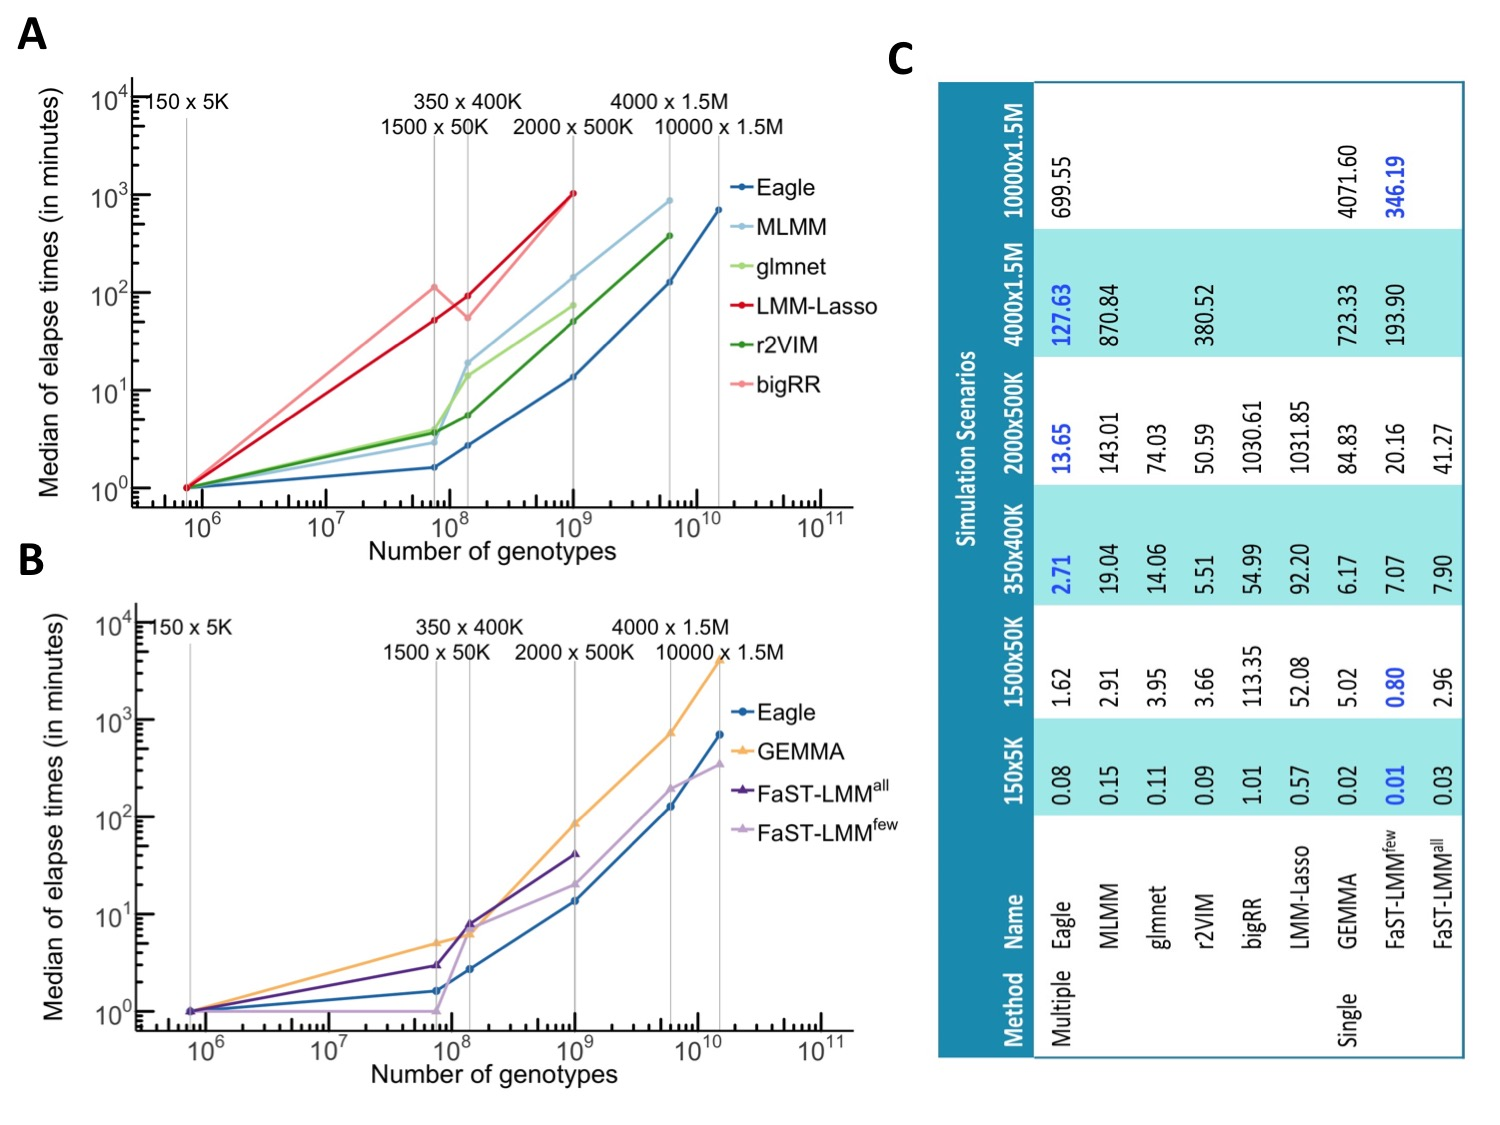
\includegraphics[width=1.0\textwidth,natwidth=610,natheight=642]{Figure2_time.jpg}
\end{figure}

 



\end{document}
